\chapter{Characterisation of Distributed Systems and System Models}

\begin{multicols*}{2}

\noindent Distributed System (DS) is a set of networked computers that communicate and coordinate their actions only by passing messages.

\noindent Internet is a very large distributed system that enables users to make use of services from everywhere

\section{Fundamental Characteristics of DS}

\noindent Concurrency: add more computers to increase capacity, and hence higher performance \\

\noindent Loosely coupled: no global clock and no global shared memory \\

\noindent Independent failures: any computer and subnetwork can fail at anytime, can be more fault-tolerant than stand-alone systems

\section {Main Motivation of DS: Resource Sharing}

\noindent Resources are shared by using services. Service is a distinct part of a computer system providing accesses to the managed resources \\

\noindent For resource sharing works, we must define:
\begin{itemize}
    \item Content and format of resources
    \item Naming and address
    \item Communication infrastructures
\end{itemize}

\section{Issues and Problems in DS}

\noindent Heterogeneity: hardware and software components are not identical, such as networks, endian formats, operating systems and programming languages\\

\noindent Scalability: remain effective when resources and users increase. This can be achieve by caching and replication of data and deploying multiple servers. We prefer decentralised design to avoid performance bottlenecks. \\

\noindent Failure handling: can be achieved by detecting, masking, tolerating, and recovery of failure

\section{Architecture Models}

\noindent Architectural model defines components, functions, placement of components, and relationship between components.

\subsection{Software and Hardware Layers}

\begin{center}
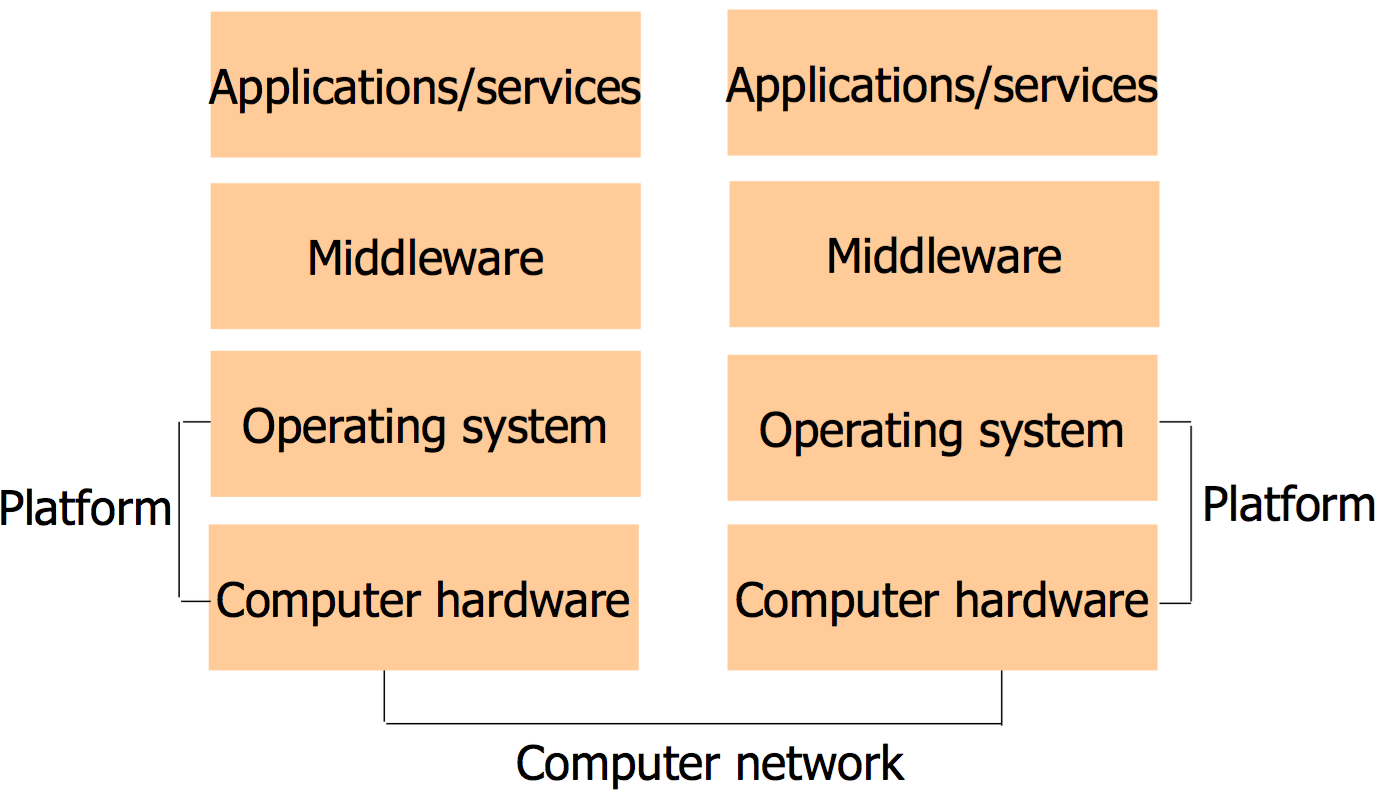
\includegraphics[width=8cm]{sw-hw-layers}
\end{center}

\noindent Platform provides system’s programming interface that facilitates communication and coordination between processes\\ 

\noindent Middleware masks heterogeneity and provide a convenient programming model. It provides generic services to application.

\subsection{Client-server Model}

\noindent $M$ servers work together for $N$ clients, so there is a division of work among $M$ servers. These servers need partitioning of data or function and replication of data or function.

\subsection{Peer-to-peer Model}

\noindent All processes play similar roles as clients and servers. They interact cooperatively as peers to perform distributed computation 

\section{Fundamental Models}

\noindent Fundamental model is formal description of common and intrinsic properties in architectural model. It makes exact claims by logical analysis and mathematical proof. 

\subsection{Interaction Model}

\noindent Synchronous distributed system assumes upper and lower bounds on processing time, transmission time, and clock drift rate. We can infer properties, such as using timeouts to detect failures.\\

\noindent Asynchronous distributed system assumes no bounds on processing time, transmission time and clock drift rate.

\subsection{Failure Model}

\noindent Failure model defines the ways in which failures may occur \\

\noindent Omission failure: a process or communication channel fails to perform actions it is supposed to do. \\

\noindent Arbitrary / Byzantine Failure: arbitrarily omit intended processing steps and take unintended processing steps.

\end{multicols*}
